\documentclass{beamer}
%Information to be included in the title page:
\title{Do cryptocurrencies extend the mean-variance frontier of an equity investor?}
\author{Sander Naerum, Thomas Pietsch and Ziga Jagodnik}
\institute{UZH}
\date{2023}

\begin{document}

\frame{\titlepage}

\begin{frame}
\frametitle{The Project}
In this project we will investigate if cryptocurrencies extend the mean-variance frontier of an equity investor. By using an industry portfolio dataset consisting of 12 different industries collected from Kenneth French data library combined with the 3 largest cryptocurrencies based on market capitalization, we extract the mean-variance frontier. We show that adding cryptocurrencies to the mean-variance frontier has a significant impact.
\end{frame}

\begin{frame}
\frametitle{Analysis}
\begin{figure}
    \centering
    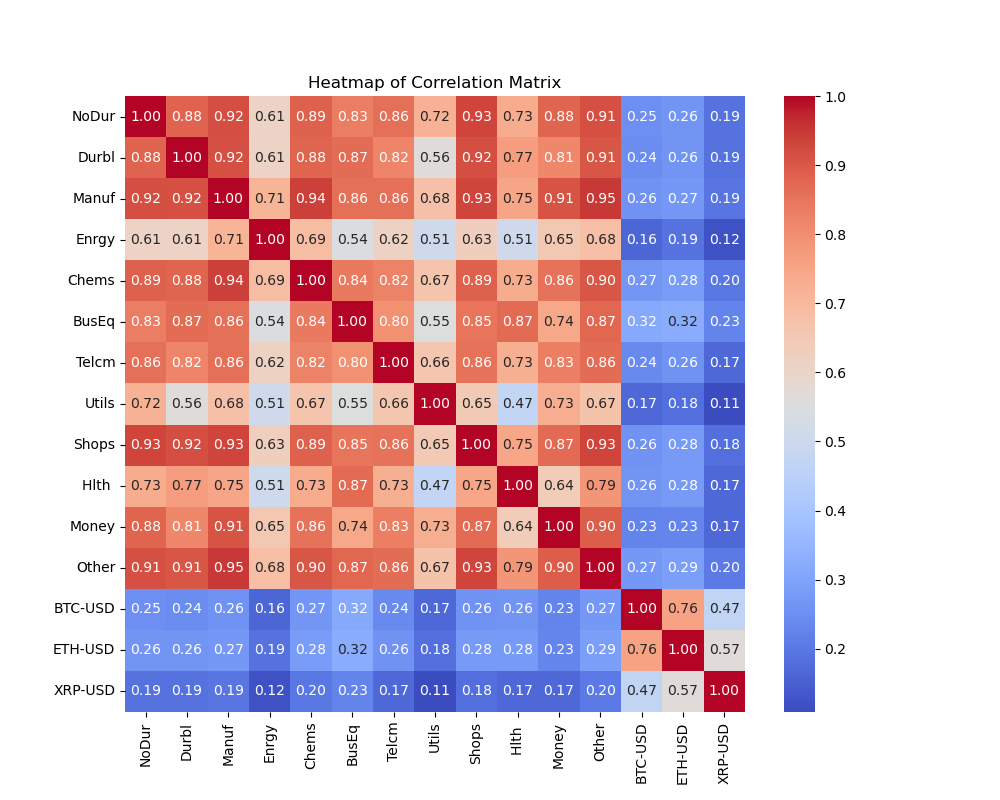
\includegraphics[width=0.8\linewidth]{Figures/heatmap_correlation.png}
    \caption{Full sample correlations}
    \label{fig:corr}
\end{figure}
\end{frame}

\begin{frame}
\frametitle{Analysis}
\begin{figure}
    \centering
    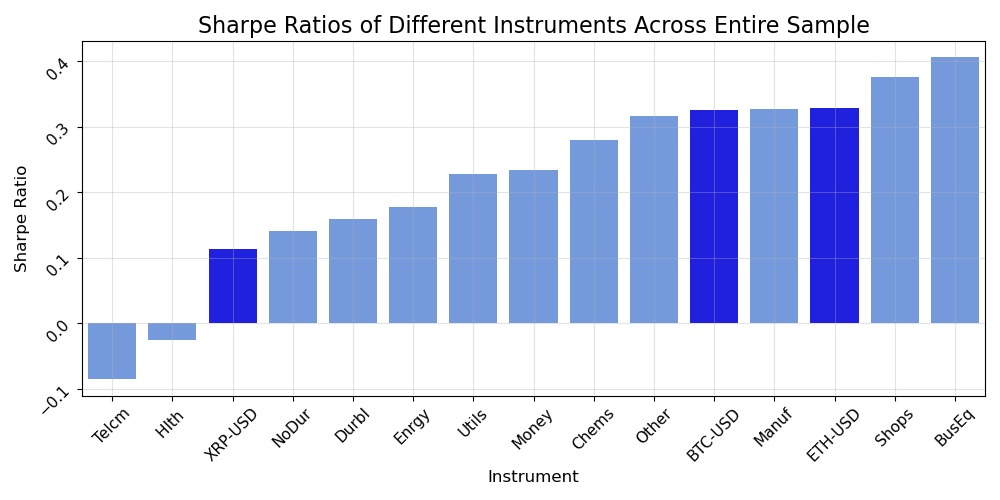
\includegraphics[width=0.8\linewidth]{Figures/SR_Entire_Sample.png}
    \caption{Full sample Sharpe's}
    \label{fig:sharpe}
\end{figure}
\end{frame}

\begin{frame}
\frametitle{Results}
\begin{figure}
    \centering
    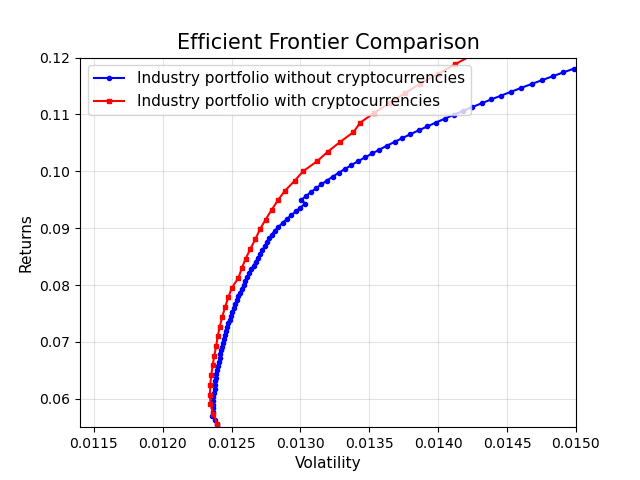
\includegraphics[width=0.8\linewidth]{Figures/Efficient_Frontier_Comparison_Full_Sample.png}
    \caption{Full sample}
    \label{fig:full}
\end{figure}
\end{frame}

\begin{frame}
\frametitle{Results}
\begin{figure}
    \centering
    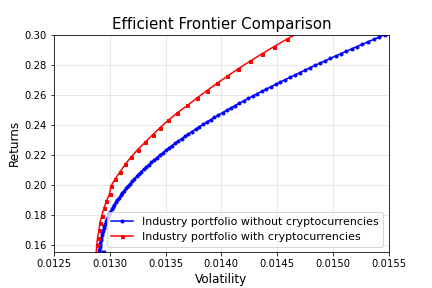
\includegraphics[width=0.8\linewidth]{Figures/Efficient_Frontier_Comparison_Bull_Market.png}
    \caption{Restricted sample}
    \label{fig:restricted}
\end{figure}
\end{frame}

\begin{frame}
\frametitle{Conclusion}
The inclusion of cryptocurrencies in an investment portfolio extends the mean-variance frontier for an equity investor, introducing a new dimension to diversification strategies and expanding the spectrum of risk and return possibilities. \nocite{wikiref}
\end{frame}

\begin{frame}
\frametitle{Bibliography}

\bibliographystyle{apalike}
\bibliography{References}
\end{frame}

\end{document}